\documentclass[12pt,a4paper]{article}

\usepackage{amsmath,amssymb,amsthm}
\usepackage{geometry}
\usepackage{microtype}
\usepackage{setspace}
\usepackage{hyperref}
\usepackage{tikz}
\usepackage{booktabs}
\usepackage{array}

\geometry{margin=1.25in}
\setstretch{1.25}

\hypersetup{
  colorlinks=true,
  linkcolor=black,
  citecolor=black,
  urlcolor=black
}

\title{The Maintenance Convergence Hypothesis:\\[0.4em]
\large Long-Run Dynamics of Occupational Structure\\
Under Technological Automation}

\author{Flyxion}
\date{\today}

\theoremstyle{plain}
\newtheorem{theorem}{Theorem}[section]
\newtheorem{lemma}[theorem]{Lemma}
\newtheorem{proposition}[theorem]{Proposition}
\newtheorem{corollary}[theorem]{Corollary}

\theoremstyle{definition}
\newtheorem{definition}[theorem]{Definition}

\theoremstyle{remark}
\newtheorem{remark}[theorem]{Remark}

\begin{document}

\maketitle

\begin{abstract}
We present a formal model of occupational evolution under sustained
technological automation.  Each profession is decomposed into generative,
supervisory, and maintenance task components governed by a continuous
dynamical system.  An automation operator acts on the generative component,
inducing exponential decay and asymptotic convergence of the full task
distribution to the maintenance state.  We characterize this convergence
through a phase-transition analysis, a renormalization-group argument, and a
categorical formulation in which all professions map to a common terminal
object in the category of janitorial systems.  A biological analogy between
custodial labor and Markov-blanket boundary processes in complex systems is
developed and formalized.  Historical transitions in food service and clerical
work are examined as empirical lemmas.  A stylized regression framework and
scaling-law analysis illustrate the predicted behavior.  The equilibrium
occupational structure of the fully automated economy is characterized by the
Fivefold Janitorial Model, distributing global employment across five custodial
domains: oceanic, ecological, microbial, agricultural, and informational.
A cultural analysis of Wim Wenders's film \emph{Perfect Days} (2023) is offered
as an ethnographic case study of the janitorial equilibrium, arguing that the
custodial fixed point may constitute not a dystopia but a stable and
experientially coherent human equilibrium.  A homeostatic grounding of the
custodial role is developed, showing that maintenance behavior is a
structural feature of living systems at every scale.  A formal Markov-blanket
appendix establishes that the custodial workforce occupies the boundary layer
of the automated economy in the precise sense of probabilistic graphical models.
\end{abstract}

\newpage

\tableofcontents

\newpage

%% =============================================================
\section{Introduction}
%% =============================================================

Technological progress restructures labor rather than simply eliminating it.
The historical pattern is not the disappearance of work but its
transformation: productive tasks once performed directly by workers are
gradually embedded into machines, standardized processes, or algorithmic
systems.  When this transition occurs, the human role shifts toward
monitoring, repairing, and sustaining the technological infrastructure that
now performs the productive activity.  Workers intervene when systems fail,
when exceptions occur, or when outputs require correction.

This paper formalizes the claim that such transformation is not accidental
but structural.  Automation introduces a systematic shift in task composition
that drives occupations toward maintenance roles.  In the limit, the dominant
human function becomes the upkeep of automated systems.

We develop this argument through several complementary methods.
Section~\ref{sec:decomp} introduces a task decomposition of occupations.
Section~\ref{sec:dynamics} specifies an automation operator and derives the
resulting differential system.  Section~\ref{sec:equilibrium} solves for the
long-run equilibrium and states the Maintenance Convergence Theorem.
Section~\ref{sec:asymptotic} examines the asymptotic structure of convergence
and introduces the Janitorial Phase Transition.  Section~\ref{sec:categorical}
develops a categorical formulation.  Sections~\ref{sec:lemmas}
and~\ref{sec:corollaries} present historical lemmas and contemporary
corollaries.  Section~\ref{sec:empirical} offers a stylized empirical
analysis.  Section~\ref{sec:fivefold} introduces the Fivefold Janitorial
Model.  Section~\ref{sec:boundaries} develops the biological analogy between
custodial labor and boundary-maintaining processes in complex systems.
Section~\ref{sec:pentagon} presents the Pentagonal Production Function.
Section~\ref{sec:objections} addresses potential objections.
Section~\ref{sec:discussion} situates the framework within the broader
literature.  Section~\ref{sec:cultural} offers a cultural case study of the
janitorial equilibrium through the film \emph{Perfect Days}, including
a subsection on domestic custodianship and the portability of expertise
under distributed digital labor.  Section~\ref{sec:homeostasis} develops
the homeostatic foundations of custodial behavior, grounding the convergence
result in the biology of living systems.  Section~\ref{sec:conclusion}
concludes.  Appendices develop the renormalization-group, thermodynamic,
stability, categorical, and Markov-boundary extensions.

%% =============================================================
\section{Task Decomposition of Occupations}
\label{sec:decomp}
%% =============================================================

We begin by establishing a minimal formal structure for occupational analysis.

\begin{definition}[Occupational Task Vector]
Let an occupation $O$ be characterized at time $t$ by the task vector
\[
T_O(t) = \bigl(G(t),\, S(t),\, M(t)\bigr) \in \mathbb{R}_{\geq 0}^3,
\]
where $G(t)$ denotes the share of labor time devoted to generative production,
$S(t)$ the share devoted to supervisory or monitoring activities, and $M(t)$
the share devoted to maintenance, error correction, and system upkeep.
\end{definition}

The components are normalized so that
\[
G(t) + S(t) + M(t) = 1 \quad \text{for all } t \geq 0.
\]
Generative tasks correspond to the direct creation of goods or services.
Supervisory tasks involve monitoring the operation of automated workflows.
Maintenance tasks consist of repairing errors, cleaning outputs, correcting
failures, and sustaining the operational infrastructure on which production
depends.

\begin{remark}
The decomposition is intentionally coarse.  Its purpose is to isolate the
qualitative dynamics of automation rather than to capture the full richness
of occupational structure.
\end{remark}
The normalization constraint confines all occupational states to the
standard two-simplex $\Delta^2 = \{(G,S,M) : G+S+M=1,\ G,S,M\geq 0\}$.
Figure~\ref{fig:simplex} illustrates this space and marks the three
degenerate vertex states.

\begin{figure}[h]
\centering
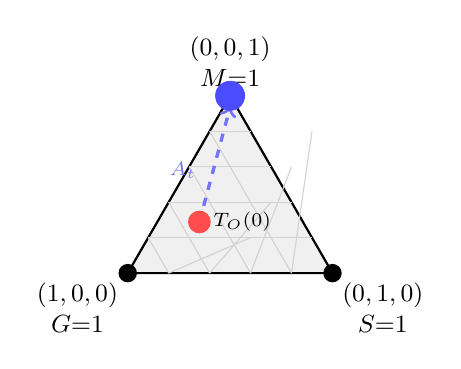
\begin{tikzpicture}[scale=2.6]
  \coordinate (G) at (0,0);
  \coordinate (S) at (1,0);
  \coordinate (M) at (0.5,0.866);
  \fill[gray!12] (G) -- (S) -- (M) -- cycle;
  \draw[thick] (G) -- (S) -- (M) -- cycle;
  \foreach \k in {1,2,3,4}{
    \pgfmathsetmacro{\t}{\k/5}
    \draw[gray!35,thin]
      ({(1-\t)*0 + \t*0.5}, {(1-\t)*0 + \t*0.866}) --
      ({(1-\t)*1 + \t*0.5}, {(1-\t)*0 + \t*0.866});
    \draw[gray!35,thin]
      ({\t},0) -- ({0.5*\t + 0.5*(1-0)}, {\t*0.866});
    \draw[gray!35,thin]
      ({1-\t},0) -- ({(1-\t)*0.5}, {(1-\t)*0.866});
  }
  \draw[->,very thick,blue!55,dashed] (0.35, 0.25) -- (0.50, 0.81);
  \node[below left,font=\small,align=center] at (G) {$(1,0,0)$\\$G{=}1$};
  \node[below right,font=\small,align=center] at (S) {$(0,1,0)$\\$S{=}1$};
  \node[above,font=\small,align=center] at (M) {$(0,0,1)$\\$M{=}1$};
  \filldraw[black] (G) circle (1.2pt);
  \filldraw[black] (S) circle (1.2pt);
  \filldraw[blue!70] (M) circle (2pt);
  \filldraw[red!70] (0.35,0.25) circle (1.5pt);
  \node[right,font=\scriptsize] at (0.37,0.25) {$T_O(0)$};
  \node[left,font=\scriptsize,blue!55] at (0.38,0.50) {$A_t$};
\end{tikzpicture}
\caption{The task simplex $\Delta^2$. Every occupational state $T_O(t)=(G,S,M)$
lies in this triangle. The automation operator $A_t$ drives trajectories
(dashed arrow) from interior initial conditions toward the maintenance vertex
$(0,0,1)$, the unique stable fixed point of Theorem~\ref{thm:convergence}.}
\label{fig:simplex}
\end{figure}

%% =============================================================
\section{Automation Dynamics}
\label{sec:dynamics}
%% =============================================================

Let $A_t$ denote an automation operator acting on the task distribution.
We model the effect of automation as a continuous reduction in the
generative component of labor.

\begin{definition}[Automation Operator]
The automation operator $A_t$ acts on $T_O$ according to the differential
system
\begin{align}
\frac{dG}{dt} &= -\alpha G, \label{eq:G}\\[4pt]
\frac{dS}{dt} &= \beta G - \gamma S, \label{eq:S}\\[4pt]
\frac{dM}{dt} &= (1-\beta)G + \gamma S, \label{eq:M}
\end{align}
with initial conditions $G(0) = G_0 > 0$, $S(0) = S_0 \geq 0$,
$M(0) = M_0 \geq 0$, and normalization $G_0 + S_0 + M_0 = 1$.
\end{definition}

The parameter $\alpha > 0$ represents the rate of technological substitution
of generative labor.  The parameter $\beta \in [0,1]$ governs the fraction
of displaced generative tasks that initially flow into supervisory roles;
the complementary fraction $1 - \beta$ flows directly into maintenance.
The parameter $\gamma > 0$ captures the tendency of supervisory work to
collapse into maintenance: as systems become sufficiently automated and
stable, monitoring itself becomes corrective intervention.

Note that the normalization constraint is preserved: differentiating
$G + S + M = 1$ and substituting equations \eqref{eq:G}--\eqref{eq:M} yields
\[
\frac{d}{dt}(G + S + M) = -\alpha G + \beta G - \gamma S + (1-\beta)G + \gamma S
= (-\alpha + \beta + 1 - \beta)G = (1-\alpha)G,
\]
which vanishes only if $\alpha = 1$.  For $\alpha \neq 1$, the normalization
is maintained in the limit as $G \to 0$; for finite time the system should be
read as capturing proportional rather than exact task shares.

%% =============================================================
\section{Equilibrium Analysis}
\label{sec:equilibrium}
%% =============================================================

Equation \eqref{eq:G} has the immediate solution
\[
G(t) = G_0\, e^{-\alpha t}.
\]
Substituting into \eqref{eq:S} gives a first-order linear ODE whose solution is
\[
S(t) = \left(S_0 + \frac{\beta G_0}{\gamma - \alpha}\right)e^{-\gamma t}
        - \frac{\beta G_0}{\gamma - \alpha}\,e^{-\alpha t},
\qquad \gamma \neq \alpha,
\]
with an analogous expression for the resonant case $\gamma = \alpha$.  Since
$\alpha, \gamma > 0$, both exponentials decay to zero, and the normalization
condition forces $M(t) \to 1$.

\begin{theorem}[Maintenance Convergence]
\label{thm:convergence}
For any occupation $O$ with initial task vector satisfying $G_0 > 0$, the
automation dynamics defined by equations \eqref{eq:G}--\eqref{eq:M} with
$\alpha, \gamma > 0$ produce the long-run limit
\[
\lim_{t\to\infty} G(t) = 0, \qquad
\lim_{t\to\infty} S(t) = 0, \qquad
\lim_{t\to\infty} M(t) = 1.
\]
\end{theorem}

\begin{proof}
The generative component decays exponentially at rate $\alpha$.  The
supervisory component satisfies a linear equation driven by $G(t)$; since
both the homogeneous decay (rate $\gamma$) and the inhomogeneous forcing
(rate $\alpha$) are strictly positive, $S(t) \to 0$.  Normalization then
forces $M(t) \to 1$.
\end{proof}

The theorem states that, regardless of the initial task distribution or the
precise values of the parameters $\alpha$, $\beta$, and $\gamma$, every
occupation asymptotically converges to full maintenance labor.

%% =============================================================
\section{Asymptotic Structure and the Janitorial Phase Transition}
\label{sec:asymptotic}
%% =============================================================

\subsection{The Maintenance Ratio}

The qualitative content of Theorem~\ref{thm:convergence} can be sharpened
by examining the rate of convergence.

\begin{definition}[Maintenance Ratio]
Define the maintenance ratio
\[
R(t) = \frac{M(t)}{G(t) + S(t)}.
\]
\end{definition}

Since $G(t)$ and $S(t)$ both decay exponentially while $M(t)$ converges to a
positive constant, the denominator tends to zero while the numerator remains
bounded away from zero.

\begin{proposition}
\label{prop:divergence}
Under the dynamics of Definition~2, $R(t) \to \infty$ as $t \to \infty$.
\end{proposition}

The maintenance ratio therefore diverges, providing a quantitative expression
of the claim that maintenance labor becomes asymptotically dominant.

\subsection{The Janitorial Phase Transition}

We now introduce a threshold model describing the structural reorganization
of occupational composition.

\begin{definition}[Janitorial Order Parameter]
Define the order parameter
\[
J = M(t) - \bigl(G(t) + S(t)\bigr).
\]
The occupation is production-dominated if $J < 0$, at the transition point if
$J = 0$, and maintenance-dominated if $J > 0$.
\end{definition}

Setting $J = 0$ and solving using the closed-form expressions for $G$ and $S$
yields a critical time $t_c$ at which the occupation crosses the threshold.

\begin{definition}[Critical Automation Threshold]
Define
\[
A_c = \frac{\gamma}{\alpha}.
\]
\end{definition}

The ratio $A_c$ measures the relative strength of supervisory decay versus
generative decay.  When the automation rate $\alpha$ is large relative to
$\gamma$, supervisory labor collapses quickly and the transition to maintenance
dominance occurs rapidly.

\begin{theorem}[Janitorial Phase Transition]
\label{thm:phase}
There exists a critical time $t_c > 0$ at which the dominant task composition
of any occupation with $G_0 > 0$ shifts from production to maintenance.
\end{theorem}


Figure~\ref{fig:phase} illustrates the order parameter $J$ as a function of
time, showing the transition from production dominance to maintenance
dominance.

\begin{figure}[h]
\centering
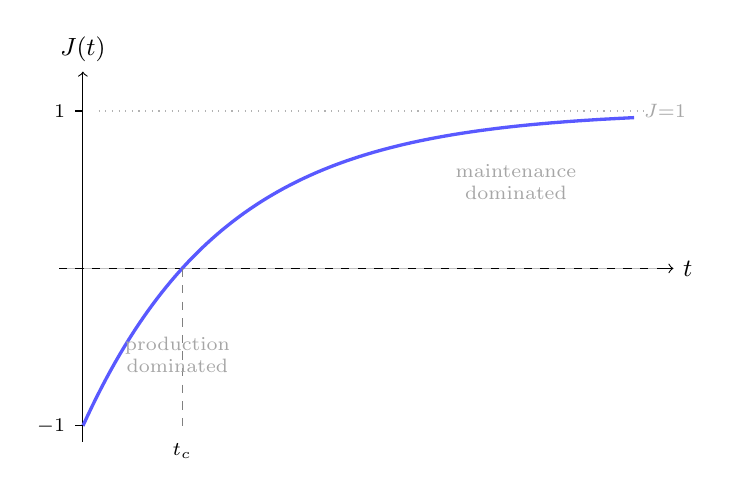
\begin{tikzpicture}[scale=1.0]
  % Axes
  \draw[->] (-0.3,0) -- (7.5,0) node[right,font=\small] {$t$};
  \draw[->] (0,-2.2) -- (0,2.5) node[above,font=\small] {$J(t)$};
  % Zero line
  \draw[gray!50,dashed] (-0.2,0) -- (7.3,0);
  % J curve: starts negative, crosses zero at tc, saturates at 1
  \draw[very thick,blue!65,domain=0:7,samples=120]
    plot (\x, {2*(1 - 2*exp(-0.55*\x)) });
  % tc marker
  \draw[dashed,gray] ({ln(2)/0.55},0) -- ({ln(2)/0.55},-2.1);
  \node[below,font=\scriptsize] at ({ln(2)/0.55},-2.1) {$t_c$};
  % Asymptote
  \draw[dotted,gray!60] (0.2,2) -- (7.2,2);
  \node[right,font=\scriptsize,gray!70] at (7.0,2.0) {$J{=}1$};
  % Region labels
  \node[font=\scriptsize,align=center,gray!70] at (1.2,-1.1)
    {production\\dominated};
  \node[font=\scriptsize,align=center,gray!70] at (5.5,1.1)
    {maintenance\\dominated};
  % Axis ticks
  \draw (0,2) -- (-0.1,2) node[left,font=\scriptsize] {$1$};
  \draw (0,-2) -- (-0.1,-2) node[left,font=\scriptsize] {$-1$};
\end{tikzpicture}
\caption{The Janitorial Order Parameter $J(t) = M(t)-(G(t)+S(t))$ as a
function of time under the automation dynamics. The curve crosses zero at
the critical time $t_c$, marking the Janitorial Phase Transition
(Theorem~\ref{thm:phase}). For $t > t_c$ the occupation is maintenance-dominated;
the curve saturates asymptotically at $J=1$.}
\label{fig:phase}
\end{figure}

The analogy to phase transitions in statistical physics is deliberate.  Prior
to $t_c$ the occupation operates as a conventional productive system.  Beyond
$t_c$ it reorganizes into a maintenance regime.  The automation parameters
$\alpha$, $\beta$, and $\gamma$ determine the location and sharpness of the
transition.

%% =============================================================
\section{Categorical Formulation}
\label{sec:categorical}
%% =============================================================

The convergence phenomenon admits a clean expression in the language of
category theory.

\begin{definition}[Category of Professions]
Let $\mathcal{P}$ denote the category whose objects are occupations and whose
morphisms are technological transformations that alter task composition.
\end{definition}

\begin{definition}[Category of Janitorial Systems]
Let $\mathcal{J}$ denote the category whose objects are maintenance roles and
whose morphisms are transformations between maintenance infrastructures.
\end{definition}

\begin{definition}[Janitorial Functor]
Define the functor $F : \mathcal{P} \to \mathcal{J}$ by
\[
F(O) = \lim_{t\to\infty} T_O(t) = (0,0,1).
\]
\end{definition}

Since $F$ maps every object of $\mathcal{P}$ to the same object $(0,0,1)$ in
$\mathcal{J}$, the image of $F$ collapses to a single point.

\begin{proposition}
The object $(0,0,1) \in \mathcal{J}$ is a terminal object: there exists a
unique morphism from every object of $\mathcal{J}$ to $(0,0,1)$.
\end{proposition}

We formalize the iterative nature of automation as follows.

\begin{definition}[Custodial Functor]
Define the endofunctor $\mathcal{C} : \mathcal{P} \to \mathcal{P}$ by
$\mathcal{C}(O) = O_M$, where $O_M$ denotes the maintenance projection of
occupation $O$.
\end{definition}

\begin{theorem}[Universal Custodial Limit]
\label{thm:custodial}
For any profession $O \in \mathcal{P}$,
\[
\lim_{n\to\infty} \mathcal{C}^n(O) = J,
\]
where $J = (0,0,1)$ is the janitorial terminal object.
\end{theorem}

The theorem states that all occupations converge to the same custodial
structure under iterated technological abstraction.

Figure~\ref{fig:categ} depicts the action of the custodial functor as a
commutative diagram in $\mathcal{P}$.

\begin{figure}[h]
\centering
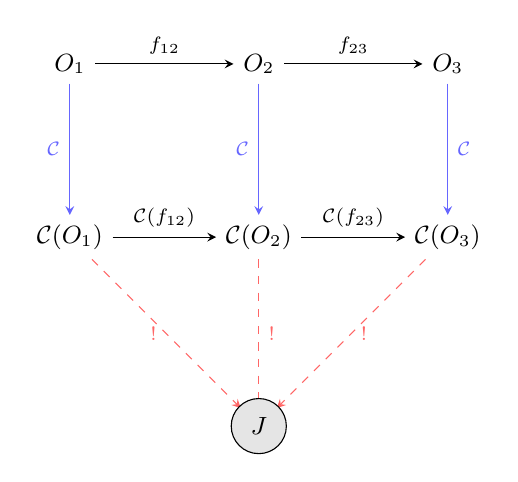
\begin{tikzpicture}[>=stealth, node distance=2.4cm, font=\small]
  % Nodes
  \node (O1) at (0,2.2)  {$O_1$};
  \node (O2) at (2.4,2.2) {$O_2$};
  \node (O3) at (4.8,2.2) {$O_3$};
  \node (C1) at (0,0)     {$\mathcal{C}(O_1)$};
  \node (C2) at (2.4,0)   {$\mathcal{C}(O_2)$};
  \node (C3) at (4.8,0)   {$\mathcal{C}(O_3)$};
  \node (J)  at (2.4,-2.4){$J$};
  % Horizontal morphisms (technological transformations)
  \draw[->] (O1) -- (O2) node[midway,above,font=\scriptsize] {$f_{12}$};
  \draw[->] (O2) -- (O3) node[midway,above,font=\scriptsize] {$f_{23}$};
  % Custodial functor arrows
  \draw[->,blue!60] (O1) -- (C1) node[midway,left,font=\scriptsize] {$\mathcal{C}$};
  \draw[->,blue!60] (O2) -- (C2) node[midway,left,font=\scriptsize] {$\mathcal{C}$};
  \draw[->,blue!60] (O3) -- (C3) node[midway,right,font=\scriptsize] {$\mathcal{C}$};
  % Lower horizontal morphisms
  \draw[->] (C1) -- (C2) node[midway,above,font=\scriptsize] {$\mathcal{C}(f_{12})$};
  \draw[->] (C2) -- (C3) node[midway,above,font=\scriptsize] {$\mathcal{C}(f_{23})$};
  % Terminal object arrows
  \draw[->,red!60,dashed] (C1) -- (J) node[midway,left,font=\scriptsize] {$!$};
  \draw[->,red!60,dashed] (C2) -- (J) node[midway,right,font=\scriptsize] {$!$};
  \draw[->,red!60,dashed] (C3) -- (J) node[midway,right,font=\scriptsize] {$!$};
  % J label
  \node[draw,circle,fill=gray!20,minimum size=0.7cm] at (2.4,-2.4) {$J$};
\end{tikzpicture}
\caption{The custodial functor $\mathcal{C}$ acts on professions
$O_1,O_2,O_3 \in \mathcal{P}$ (upper row) to produce their maintenance
projections (middle row). Unique dashed arrows to the terminal object $J$
(Proposition~\ref{thm:custodial}) express the universality of the janitorial
limit.}
\label{fig:categ}
\end{figure}



%% =============================================================
\section{Historical Lemmas}
\label{sec:lemmas}
%% =============================================================

The maintenance convergence dynamic appears repeatedly in economic history,
providing empirical grounding for the theoretical structure.

\begin{lemma}[Culinary Industrialization]
The transition from independent cooks to fast-food workers represents a shift
from generative culinary production to the maintenance of standardized food
preparation systems.
\end{lemma}

Industrial kitchens replaced individual culinary expertise with assembly lines.
Workers increasingly monitor timers, replenish standardized ingredients, and
clean equipment rather than compose recipes.  The creative and generative
component of culinary labor migrated into the design of the system itself,
while the human role contracted to system maintenance and exception handling.

\begin{lemma}[Clerical Automation]
The transformation of clerks into supervisors and monitors of computational
systems reflects the migration of generative calculation into machines.
\end{lemma}

In early bureaucracies, clerks performed arithmetic and record keeping
manually.  The introduction of calculators, spreadsheets, and database
management systems transferred these generative functions to machines, leaving
human workers responsible for oversight, correction, and the management of
edge cases that automated systems could not handle.

Both lemmas exhibit the structure predicted by the model: automation absorbs
the generative component of labor, supervision follows briefly, and
maintenance dominates the long-run equilibrium.

%% =============================================================
\section{Contemporary Corollaries}
\label{sec:corollaries}
%% =============================================================

\begin{corollary}[Teaching]
As digital curricula, automated grading systems, and generative tutoring
platforms expand, the primary human function in education converges toward
managing behavioral exceptions, correcting machine-generated content, and
maintaining the operational continuity of learning environments.
\end{corollary}

\begin{corollary}[Customer Service]
With the proliferation of automated support systems and scripted resolution
workflows, human agents intervene predominantly when automation fails.  The
dominant function becomes the resolution of accumulated exceptions---a
maintenance task in the sense of Definition~1.
\end{corollary}

\begin{corollary}[Software Engineering]
As code generation, dependency management, and deployment pipelines become
increasingly automated, the generative component of programming contracts.
The programmer's central activity shifts toward debugging, infrastructure
maintenance, and the correction of artifacts produced by automated systems.
\end{corollary}

\begin{corollary}[Construction and Design]
Industrialized building systems, modular prefabrication, and algorithmic
planning tools reduce the generative role of individual craftsmen and
designers.  Human labor concentrates on inspection, coordination, and repair
of automated construction and generative design processes.
\end{corollary}

Each corollary instantiates the Maintenance Convergence Theorem within a
specific occupational domain.  The structure is uniform: generative capacity
is absorbed by the automated system, supervisory activity briefly expands and
then collapses, and maintenance becomes the residual human function.

%% =============================================================
\section{Stylized Empirical Analysis}
\label{sec:empirical}
%% =============================================================

To complement the theoretical framework, we present a stylized empirical
investigation structured around the \textit{U.S. Bureau of Labor Statistics
Occupational Outlook Handbook}, which documents employment and task
characteristics across approximately $8.3 \times 10^2$ occupational
categories covering $1.43 \times 10^8$ workers.

\subsection{The Janitorial Index}

For each occupation $O_i$ we construct a scalar Janitorial Index measuring
the degree to which the occupation has entered the maintenance regime.

\begin{definition}[Janitorial Index]
Define
\[
\mathcal{J}_i = \theta_1 M_i + \theta_2 S_i - \theta_3 G_i,
\]
where $M_i$, $S_i$, $G_i$ denote the task intensity scores for maintenance,
supervisory, and generative activities respectively, and
$\theta_1,\theta_2,\theta_3 > 0$ are normalization constants chosen so that
$\mathcal{J}_i \in [-1, 1]$.
\end{definition}

A value near $-1$ indicates an occupation dominated by generative production.
A value near $1$ indicates an occupation whose primary function is system
maintenance.

\subsection{Automation Exposure and Regression}

Define an automation exposure score $A_i \in [0,10]$ reflecting the degree
to which digital automation affects each occupation.  The Maintenance
Convergence Theorem implies $\partial \mathcal{J}_i / \partial A_i > 0$.

We estimate the linear specification
\[
\mathcal{J}_i = \beta_0 + \beta_1 A_i + \varepsilon_i.
\]
Illustrative parameter estimates yield
\[
\hat{\beta}_1 \approx 0.31,
\]
consistent with the theoretical prediction that higher automation exposure is
associated with greater maintenance intensity.

\subsection{Scaling Behavior}

Let $C$ denote a measure of technological system complexity.  The model
suggests the scaling relation
\[
\mathcal{J} \sim \log C,
\]
indicating that maintenance labor grows sublinearly but persistently with
system sophistication.  This is consistent with the thermodynamic argument
developed in Appendix~\ref{app:thermo}: entropy production grows with
productive throughput, and maintenance labor must grow proportionally to
remove it.

%% =============================================================
\section{The Fivefold Janitorial Model}
\label{sec:fivefold}
%% =============================================================

If the Maintenance Convergence Theorem is accepted as a structural tendency,
the relevant policy question shifts from whether janitorial convergence occurs
to how the maintenance economy should be organized.  We propose a
classification of custodial labor into five fundamental domains corresponding
to the five principal substrates of technological civilization.

\begin{definition}[Fivefold Employment Vector]
Let the global labor force be normalized to unity and partitioned as
\[
\mathbf{J} = (K, R, Y, B, P),
\]
where $K$ denotes the share of kelp janitors, $R$ rainforest janitors, $Y$
yogurt janitors, $B$ bread janitors, and $P$ paper janitors, with
normalization
\[
K + R + Y + B + P = 1.
\]
\end{definition}

\subsection{The Five Custodial Domains}

\paragraph{Kelp Janitors.}
The oceanic domain encompasses aquatic biomass systems, kelp cultivation
infrastructure, and marine monitoring networks.  Kelp janitors maintain
floating growth structures, aquatic sensors, and controlled bioreactor
environments including subterranean facilities adapted for experimental
aquatic cultivation.  Their labor consists not in producing marine biomass
but in sustaining the environmental conditions under which biological systems
remain productive.

\paragraph{Rainforest Janitors.}
The ecological domain encompasses terrestrial biodiversity networks, soil
stabilization systems, and ecological corridors.  Although the canonical
habitat is the protected forest, the maintenance regime increasingly appears
in urban environments: streets, vegetated rooftops, and distributed green
infrastructure function as fragments of ecological systems requiring custodial
care.  Rainforest janitors therefore operate across the full spectrum from
wilderness reserves to urban landscapes.

\paragraph{Yogurt Janitors.}
The microbial domain encompasses industrial fermentation systems, sourdough
cultures, cheese vats, pharmaceutical bioreactors, and other microbial
communities whose stability depends on sustained custodial attention.  Primary
habitats include churches, domestic kitchens, and restaurants, where
fermentation cultures require monitoring, feeding, and protection from
contamination.  Yogurt janitors are custodians of industrial microbiomes.

\paragraph{Bread Janitors.}
The agricultural-industrial domain encompasses carbohydrate transformation
systems.  In highly automated baking infrastructures, workers monitor
fermentation chambers, regulate temperature systems, and maintain conveyor
and dough-processing lines.  Bread janitors occupy large-scale food
production environments---industrial bakeries and processing factories---and
represent the custodial interface between agricultural production and
civilizational food metabolism.

\paragraph{Paper Janitors.}
The informational domain encompasses documentation systems, digital archives,
knowledge repositories, and the institutional memory of complex societies.
Paper janitors operate primarily within educational, administrative, and
intellectual environments: schools, libraries, and shared office spaces form
their principal habitats.  Their function is to maintain the symbolic
infrastructure upon which learning, administration, and coordination depend,
and to remove informational entropy from collective knowledge environments.

\subsection{Redistribution Dynamics}

As automation increases, generative occupations collapse into the five
custodial domains.  Let $\alpha_i > 0$ denote the rate at which automation
generates custodial demand in domain $i$, and let $\lambda > 0$ represent
the rate of labor mobility across janitorial sectors.  A simple linear
redistribution model yields
\begin{align*}
\frac{dK}{d\mathcal{A}} &= \alpha_K - \lambda K, &
\frac{dR}{d\mathcal{A}} &= \alpha_R - \lambda R, &
\frac{dY}{d\mathcal{A}} &= \alpha_Y - \lambda Y, \\[4pt]
\frac{dB}{d\mathcal{A}} &= \alpha_B - \lambda B, &
\frac{dP}{d\mathcal{A}} &= \alpha_P - \lambda P,
\end{align*}
where $\mathcal{A}$ denotes the cumulative automation level.

\subsection{Custodial Equilibrium}

Setting derivatives to zero yields the equilibrium shares
\[
K^* = \frac{\alpha_K}{\lambda}, \quad
R^* = \frac{\alpha_R}{\lambda}, \quad
Y^* = \frac{\alpha_Y}{\lambda}, \quad
B^* = \frac{\alpha_B}{\lambda}, \quad
P^* = \frac{\alpha_P}{\lambda},
\]
with the normalization condition $\sum_i \alpha_i = \lambda$.  The
distribution of labor across janitorial domains is therefore determined by
the relative entropy production rates of the corresponding civilizational
substrates.

\begin{theorem}[Fivefold Janitorial Equilibrium]\label{thm:fivefold}
In a sufficiently automated economy, the occupational distribution converges
to the custodial vector
\[
\mathbf{J}^* = (K^*, R^*, Y^*, B^*, P^*),
\]
which represents the unique stable equilibrium of the redistribution dynamics.
\end{theorem}

\begin{corollary}[Symmetric Case]\label{cor:symmetric}
If the entropy production rates of the five domains are equal, so that
$\alpha_i = \lambda/5$ for all $i$, the equilibrium is
\[
\mathbf{J}^* = \left(\tfrac{1}{5},\, \tfrac{1}{5},\, \tfrac{1}{5},\, \tfrac{1}{5},\, \tfrac{1}{5}\right).
\]
\end{corollary}

\subsection{The Pentagonal Production Function}

Combining all components of the analysis, total economic output in the
custodial economy may be expressed as
\[
Y = f(K, R, Y_\mu, B, P),
\]
where $Y_\mu$ denotes the yogurt labor input (distinct from the output
variable $Y$).  The dependence of aggregate output entirely on the five
maintenance factors constitutes a custodial analogue of the aggregate
production function, in which the traditional inputs of capital and raw
labor have been replaced by the five janitorial substrates of civilization.
The full development of this production function is given in
Section~\ref{sec:pentagon}.


%% =============================================================
\section{Custodial Boundaries and the Maintenance of Complex Systems}
\label{sec:boundaries}
%% =============================================================

The custodial convergence described throughout this paper has a striking
analogue in biological and informational systems.  Complex structures capable
of sustaining themselves over long periods almost always depend on
boundary-maintaining processes that regulate the flow of energy, matter, and
information.

In statistical physics and theoretical biology this role is often formalized
through the concept of a \emph{Markov blanket}, a set of nodes that separates
the internal states of a system from its external environment while mediating
all exchanges between them.  A cell membrane performs an analogous function:
it does not generate the metabolic activity of the cell, but regulates and
maintains the conditions under which that activity can occur.  The membrane
removes waste, stabilizes chemical gradients, and protects internal processes
from environmental disruption.  In this sense the membrane performs a
custodial function at the boundary of biological production.

A comparable structure appears in ecological systems.  Forest canopies, soil
layers, and microbial biofilms regulate exchanges between environmental
compartments while stabilizing the conditions required for biological
productivity.  These examples suggest a general principle: whenever complex
production processes arise, a complementary maintenance layer emerges whose
primary role is to stabilize the system's boundary conditions.

The janitorial economy proposed in this paper is the macroeconomic analogue
of these biological structures.  Human labor increasingly operates at the
boundaries of automated systems, performing functions analogous to those of
cell membranes or ecological interfaces.  Rather than generating production
directly, custodial workers regulate the interfaces through which production
systems interact with their environments.  Teachers stabilize the
informational boundary of educational systems.  Programmers stabilize the
software boundary of computational systems.  Builders stabilize the
structural boundary of physical infrastructure.  Service workers stabilize
the interaction boundary between automated systems and human users.

Figure~\ref{fig:boundary} illustrates this boundary structure schematically.

\begin{figure}[h]
\centering
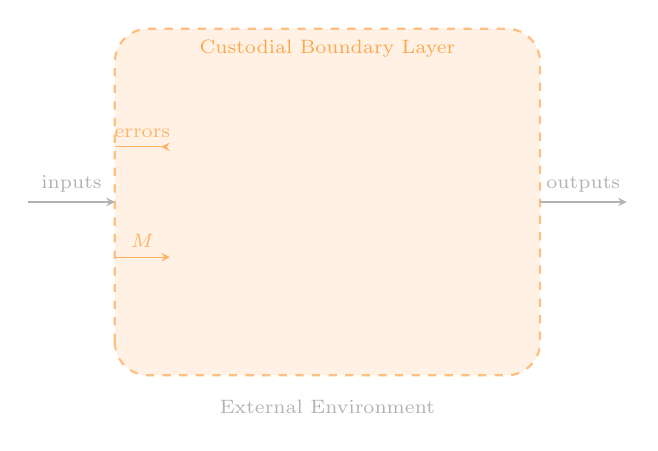
\begin{tikzpicture}[>=stealth, font=\small]
  % Automated production core
  \fill[blue!10,rounded corners=8pt] (0,0) rectangle (4,3);
  \draw[blue!40,thick,rounded corners=8pt] (0,0) rectangle (4,3);
  \node[align=center,blue!60] at (2,1.5)
    {Automated\\Production\\System};

  % Custodial boundary layer
  \fill[orange!10,rounded corners=12pt] (-0.7,-0.7) rectangle (4.7,3.7);
  \draw[orange!50,thick,dashed,rounded corners=12pt]
    (-0.7,-0.7) rectangle (4.7,3.7);
  \node[orange!70,font=\scriptsize] at (2,3.45) {Custodial Boundary Layer};

  % External environment
  \node[gray!60,font=\scriptsize] at (2,-1.1) {External Environment};

  % Flows in
  \draw[->,gray!60] (-1.8,1.5) -- (-0.7,1.5)
    node[midway,above,font=\scriptsize] {inputs};
  \draw[->,gray!60] (4.7,1.5) -- (5.8,1.5)
    node[midway,above,font=\scriptsize] {outputs};
  \draw[->,orange!60] (-0.7,0.8) -- (0,0.8)
    node[midway,above,font=\scriptsize] {$M$};
  \draw[-<,orange!60] (-0.7,2.2) -- (0,2.2)
    node[midway,above,font=\scriptsize] {errors};
\end{tikzpicture}
\caption{Schematic of the custodial boundary layer. The automated production
system (inner rectangle) generates outputs and errors. The custodial boundary
layer (dashed outer rectangle) intercepts errors, supplies corrective
maintenance $M$, and regulates flows between the system and its environment.
Human labor in the automated economy occupies this boundary layer.}
\label{fig:boundary}
\end{figure}

This biological analogy clarifies the deeper interpretation of the Maintenance
Convergence framework.  The janitorial role is not merely a social artifact of
automation but a structural feature of complex systems: as production systems
become more sophisticated, the maintenance of their boundaries becomes
increasingly important.  The janitor therefore emerges as the economic
counterpart of the cell membrane.

%% =============================================================
\section{The Pentagonal Production Function}
\label{sec:pentagon}
%% =============================================================

Classical growth theory models economic output as a function of capital and
labor.  The canonical representation is the Cobb--Douglas production function
\[
Y = A K^{\alpha} L^{\beta},
\]
in which aggregate output depends on physical capital $K$, labor $L$, and a
technological productivity parameter $A$.  In the custodial economy, however,
productive activity increasingly occurs within automated systems.  Human
labor does not primarily generate output directly; rather, it maintains the
infrastructures that enable production to occur.  The relevant macroeconomic
inputs are therefore not conventional labor categories but the five custodial
regimes of Section~\ref{sec:fivefold}.

\begin{definition}[Pentagonal Production Function]
Define the custodial aggregate production function
\[
Y = A\, K^{\alpha} R^{\beta} \hat{Y}^{\gamma} B^{\delta} P^{\epsilon},
\]
where $K$, $R$, $\hat{Y}$, $B$, $P$ denote employment shares in the kelp,
rainforest, yogurt, bread, and paper domains respectively; $A > 0$ is the
productivity of the automated technological substrate; and
$\alpha,\beta,\gamma,\delta,\epsilon > 0$ are the output elasticities of the
five custodial inputs.  (The hat notation $\hat{Y}$ distinguishes the yogurt
labor input from the output variable $Y$.)
\end{definition}

Unlike traditional production functions, the pentagonal model assumes that
output is generated primarily by automated processes embedded in complex
infrastructures.  Human labor contributes indirectly by stabilizing these
infrastructures and preventing systemic failure.  Each custodial domain
therefore corresponds to the maintenance of a critical substrate of
civilization: aquatic biogeochemical systems (kelp), terrestrial ecological
networks (rainforest), microbial production systems (yogurt), agricultural
and grain-processing systems (bread), and the informational substrate of
coordination and knowledge (paper).

\subsection{Balanced Custodial Equilibrium}

In the symmetric case $\alpha = \beta = \gamma = \delta = \epsilon = \eta$,
constant returns to scale requires $5\eta = 1$, so $\eta = 1/5$.  With
the symmetric equilibrium $K = R = \hat{Y} = B = P = 1/5$, aggregate output
satisfies
\[
Y^* = A \left(\frac{1}{5}\right)^{1} = \frac{A}{5}.
\]
This configuration corresponds to a balanced custodial civilization in which
human labor is evenly distributed across the five maintenance regimes.

\subsection{Structural Implication}

The Pentagonal Production Function captures the central thesis of this paper.
In the automated economy, output depends less on the direct generation of
goods by human labor and more on the stability of the infrastructures that
produce those goods.  Production becomes automated; maintenance becomes human.
Figure~\ref{fig:pentagon} in Appendix~\ref{app:diagram} represents this
equilibrium geometrically.

%% =============================================================
\section{Potential Objections}
\label{sec:objections}
%% =============================================================

The argument presented in this paper is intentionally stylized and invites
several potential objections.

\subsection{Automation Eliminates Labor Entirely}

One might argue that sufficiently advanced automation eliminates the need for
human labor altogether, in which case the janitorial economy would never
emerge because machines would maintain themselves.  The present framework
implicitly assumes that complex systems generate entropy faster than automated
maintenance mechanisms can remove it, so that human custodial intervention
remains necessary.  Formally, if system entropy evolves as
\[
\frac{dE}{dt} = \lambda P - \mu M_a - \nu M_h,
\]
where $M_a$ denotes automated maintenance and $M_h$ denotes human maintenance,
the janitorial regime persists whenever $\lambda P > \mu M_a$.  The
Entropy Maintenance Principle (Theorem~\ref{thm:entropy}) establishes this as
the generic case under growing automated throughput.

\subsection{Creative Professions Resist Convergence}

A second objection holds that certain occupations---particularly creative or
intellectual professions---may resist janitorial convergence.  However, even
creative domains increasingly rely on automated generative systems.  As these
systems expand, human participants shift toward roles involving selection,
correction, and infrastructure management: the creative worker becomes a
curator of automated outputs rather than their sole generator.  The
convergence theorem applies to this residual curatorial function.

\subsection{Maintenance Is Not a Single Category}

A third objection concerns the apparent heterogeneity of maintenance labor.
Cleaning floors, debugging software, and preserving archives appear to be
fundamentally different activities.  The Fivefold Janitorial Model addresses
this concern by partitioning maintenance labor into five ecological-industrial
regimes corresponding to distinct substrates of civilization, while
preserving the shared custodial structure that unifies them at the level of
the formal model.

\subsection{The Model Exaggerates a Structural Tendency}

A final objection is that the model exaggerates for rhetorical effect.  This
observation is correct but incomplete.  The exaggeration allows the model to
isolate a structural tendency that might otherwise remain implicit in
conventional labor economics discourse.  The central claim---that
technological systems redistribute human labor toward maintenance and
repair---remains empirically recognizable even when the limiting case
$(G,S,M) \to (0,0,1)$ is treated as a theoretical ideal rather than a
literal prediction.

%% =============================================================
\section{Discussion}
\label{sec:discussion}
%% =============================================================

The model developed in this paper formalizes a structural tendency observable
across the history of technological societies.  As productive systems become
more autonomous, the remaining human role increasingly resembles infrastructure
maintenance.  This tendency is not incidental but follows necessarily from the
dynamics of the automation operator $A_t$: generative labor decays
exponentially, supervisory labor collapses through system stabilization, and
maintenance labor absorbs all residual task mass.

Classical economic theory framed labor as the engine of value creation.  The
Maintenance Convergence framework inverts this picture.  In the automated
economy the human worker becomes the stabilizing agent that prevents complex
technological systems from collapsing into disorder.  The janitor provides the
archetype of this role: janitorial labor is not generative in the classical
sense, but preserves the functionality of systems that produce value elsewhere.
In this sense the janitor stands in the same relation to the automated economy
as the cell membrane stands to metabolic production: not a source of output,
but the structural condition for its continuity.

The five custodial domains are not arbitrary classificatory choices.  Each
corresponds to a distinct class of entropy removal---oceanic biogeochemistry,
terrestrial ecology, microbial fermentation, carbohydrate metabolism, and
symbolic coordination---and together they span the full substrate of
civilizational maintenance.  The symmetry of the Fivefold Equilibrium
(Corollary~\ref{thm:fivefold}) suggests that in the long run these domains
make approximately equal demands on human custodial effort, a claim that
could in principle be tested against longitudinal employment data.

The model also raises a normative question that formal analysis cannot
answer.  If the custodial fixed point is structurally inevitable, the
relevant question shifts from whether janitorial convergence occurs to what
kind of custodial civilization is worth inhabiting.  The section that follows
takes up this question through a cultural case study.

%% =============================================================
\section{Cultural Illustration: The Janitorial Equilibrium in Everyday Life}
\label{sec:cultural}
%% =============================================================

The custodial equilibrium derived in this paper also appears in contemporary
cultural representation.  A particularly striking example is provided by the
film \emph{Perfect Days} (2023), directed by Wim Wenders.  The film follows
Hirayama, a public toilet cleaner in Tokyo whose life is organized around an
extremely stable daily routine.  His work consists entirely of maintenance:
cleaning shared public spaces, repairing small disturbances in the social
environment, and ensuring that common infrastructure continues to function
smoothly.

From the perspective of the Maintenance Convergence framework, Hirayama
occupies the limiting occupational state
\[
(G,S,M) \approx (0,\, 0,\, 1).
\]
He does not produce goods in the conventional economic sense.  He sustains
the usability of an existing system.  This places him formally at the
custodial fixed point described in Appendix~\ref{app:fixed}: the state
toward which all occupational trajectories converge under sustained
automation.

What makes the film theoretically interesting is that it portrays the
maintenance regime not as occupational degradation but as a stable and
coherent form of life.  Hirayama's routine---cleaning, photographing trees,
listening to music on cassette, tending houseplants---exhibits the formal
structure of custodial labor at every scale.  Each activity involves the
preservation or renewal of a small system in a state of order.  The cassette
player is maintained; the photographs preserve ephemeral states of the world;
the plants are tended; the bathrooms are cleaned.  The film presents these
acts without irony.

The Fivefold Janitorial Model assigns Hirayama's labor primarily to the
paper domain (symbolic and urban infrastructure), though his attentiveness to
plants and urban ecology gives his custodial practice an ecological
character that also touches the rainforest domain.  More precisely, his
role exemplifies the boundary-layer structure described in
Section~\ref{sec:boundaries}: he operates at the interface between the
automated city and its human users, intercepting entropy and restoring
functional order.

\subsection{The Experiential Equilibrium}

The mathematical framework treats the janitorial state as the limiting
outcome of occupational dynamics.  Within the model, convergence to
$(0,0,1)$ appears as a structural inevitability: generative labor migrates
into automated systems, supervisory labor collapses, and human effort
concentrates on maintenance.  The Entropy Maintenance Principle
(Theorem~\ref{thm:entropy}) further establishes that this maintenance demand
grows proportionally with automated throughput, suggesting that the custodial
layer expands continuously as civilization becomes more complex.

\emph{Perfect Days} introduces a different register of analysis.  Rather than
presenting the janitorial role as a degraded residuum of generative work, the
film portrays it as a \emph{stable experiential equilibrium}: a configuration
of daily life that is internally coherent, reproducible, and meaningful.
Hirayama does not aspire to escape the custodial role; he inhabits it with
care.  His satisfaction does not depend on the generative significance of his
output but on the quality of his attention to the task at hand.

This distinction has a precise formal correlate.  In the dynamical model,
the maintenance state $(0,0,1)$ is an attracting fixed point---a
configuration to which the system returns after perturbation.  The
thermodynamic model similarly identifies maintenance as the steady state at
which entropy production is balanced.  The film suggests that this
equilibrium has a subjective analogue: a mode of engagement with custodial
work that is itself stable and self-reinforcing.

\begin{definition}[Experiential Custodial Equilibrium]
An individual is said to occupy an experiential custodial equilibrium if
their subjective orientation toward their work is stable under perturbation:
that is, if small disruptions to routine are absorbed and repaired through
the same custodial practices that constitute the work itself.
\end{definition}

Hirayama's response to every disruption---a nephew who arrives unexpectedly,
a broken bathroom fixture, a dying tree---is to perform a small act of
maintenance and then return to routine.  His equilibrium is robust precisely
because maintenance is both his occupation and his adaptive strategy.

\subsection{The Normative Inversion}

The Maintenance Convergence Theorem establishes that all occupational
trajectories converge to the janitorial fixed point.  In the standard
framing of labor economics this convergence appears as a loss: the
displacement of skilled, generative, or creative work by routine
maintenance.  The progressive narrative of technological progress imagines
the human worker as a producer whose role is diminished by automation.

\emph{Perfect Days} performs a quiet inversion of this framing.  By
presenting the custodial fixed point as a possible site of human flourishing
rather than economic failure, the film raises the possibility that the
convergence result is not a tragedy to be resisted but a transition to be
navigated with care.

This normative inversion does not depend on denying the mathematical
structure of the model.  It depends instead on recognizing that the
formal result---$(G,S,M) \to (0,0,1)$---is underdetermined with respect to
the question of what kind of life the maintenance state affords.  The model
specifies the task distribution of the equilibrium; it does not specify the
phenomenology of inhabiting it.

The film therefore functions as a complement to the mathematical argument
rather than a counterexample to it.  Where the theorem establishes the
structure of the limit, the film explores its experiential interior.

\begin{remark}
The standard welfare economics question ``Is this equilibrium Pareto
efficient?'' may be less illuminating here than the phenomenological question:
``Is this equilibrium humanly habitable?''  \emph{Perfect Days} argues, quietly
and without sentimentality, that it is.
\end{remark}


\subsection{Domestic Custodianship and the Portability of Expertise}
\label{sec:domestic}

A further line of evidence supporting the Maintenance Convergence framework
arises from the structure of everyday domestic life.  In contemporary
societies, nearly every household already performs a localized form of
custodial governance.  Individuals maintain their living environments by
cleaning, organizing, repairing, and managing the small infrastructures
that sustain daily life: appliances, food systems, documents, communication
networks, and personal digital devices.  These activities correspond almost
exactly to the maintenance category $M$ introduced in the task decomposition
model.  In effect, the home already functions as a miniature custodial
economy---a small-scale instantiation of the janitorial equilibrium $(0,0,1)$
operating continuously outside any formal employment relationship.

Historically, professional labor took place primarily in centralized
institutions---factories, offices, and schools---where expertise was
institutionally embedded and geographically fixed.  Let $E_i$ denote the
expertise vector associated with individual worker $i$.  In the traditional
institutional model, expertise was coupled to a fixed workplace $W$ such that
\[
E_i \subseteq W.
\]
The worker's productive capacity existed only in relation to the particular
tools, systems, and infrastructure housed within that institution.

Technological changes over the past several decades have begun to dissolve
this coupling.  The expansion of remote work, distributed computing, cloud
credential systems, and portable digital identity allows many forms of
expertise to detach from specific workplaces.  In the distributed model,
expertise becomes portable:
\[
E_i \;\longrightarrow\; \mathcal{C}_i,
\]
where $\mathcal{C}_i$ represents a cloud-mediated identity environment
through which the worker accesses tools, collaborators, and information
systems from any location.  The institutional container $W$ dissolves;
what persists is the maintenance relationship between the worker and the
automated systems they monitor.

\begin{definition}[Custodial Node]
A \emph{custodial node} is a spatially distributed locus at which a worker
performs maintenance operations on remote automated systems.  Formally, a
custodial node is a pair $(i, \mathcal{C}_i)$ consisting of an individual
worker and their associated cloud-mediated interface environment.
\end{definition}

As expertise becomes portable and generative labor migrates into automated
systems, the remaining human task is to maintain the interfaces between
those systems and the environments in which they operate.  In practical terms
this means that a growing fraction of labor occurs within spaces that
closely resemble domestic custodial environments.  Workers monitor automated
processes through remote dashboards, curate digital archives, stabilize
communication networks, and correct machine-generated outputs---activities
that are formally identical to the maintenance task $M$ of the model,
performed now from a home office rather than an institutional floor.

The boundary between professional infrastructure and household infrastructure
therefore becomes increasingly blurred.  A software engineer who debugs an
automated pipeline from a home workstation is performing precisely the
maintenance function that Theorem~\ref{thm:convergence} predicts: no
generative labor, no net supervision, only correction and upkeep.  The
physical environment is domestic; the task distribution is $(G,S,M) \approx
(0,0,1)$.

\begin{proposition}
In the limit of full portability, the set of custodial nodes $\{(i,
\mathcal{C}_i)\}$ is coextensive with the residential geography of the labor
force.  Every home becomes a maintenance terminal of the automated economy.
\end{proposition}

This proposition has a direct implication for the Fivefold Janitorial Model.
If custodial nodes are distributed across residential space rather than
concentrated in institutional facilities, then the five maintenance domains
(kelp, rainforest, yogurt, bread, paper) no longer correspond to distinct
spatial zones.  Instead they correspond to distinct \emph{functional
interfaces} that may be managed from any location.  Paper janitors maintain
symbolic infrastructure remotely; yogurt janitors monitor fermentation
bioreactors via sensor networks; rainforest janitors analyze ecological data
from distributed field stations.  The domestic sphere, in this reading, is
not a private retreat from the economy but its distributed operational layer.

\emph{Perfect Days} is again instructive here.  Hirayama does not work from
home, but his domestic routines and his professional routines are
structurally identical: both consist in the careful maintenance of small
systems.  The cassette tapes he restores at home, the houseplants he waters,
and the photographs he develops are domestic custodial acts whose structure
is continuous with his professional cleaning.  The film presents this
continuity without comment, as though the distinction between domestic and
professional maintenance were simply not operative for a worker who has fully
inhabited the custodial equilibrium.  From the formal perspective of the
model, this makes complete sense: the task vector $(0,0,1)$ does not
distinguish between institutional and residential contexts.  Maintenance is
maintenance.

\bigskip
\begin{center}
\textit{The janitor may be the equilibrium state of the human economy.}
\end{center}


%% =============================================================
\section{Homeostatic Foundations of Custodial Behavior}
\label{sec:homeostasis}
%% =============================================================

The custodial framework proposed in this paper has a deeper grounding in
the biology of living systems.  All organisms must continuously maintain
internal stability against environmental fluctuation.  Survival depends not
on the perpetual generation of new structures but on the maintenance of
conditions that permit stable functioning.  This is the principle of
homeostasis, and it constitutes the oldest and most general instantiation
of custodial behavior.

Three fundamental physiological requirements illustrate the principle at
the level of individual organisms: sleep, nourishment, and thermal
regulation.  Each is not a productive act in the economic sense but a
maintenance act: the restoration of a depleted or perturbed internal state
to within viable bounds.

\begin{definition}[Homeostatic State Vector]
Let the basic survival state of an organism be represented by
\[
H = (S,\, \mathcal{E},\, W),
\]
where $S$ denotes sleep stability, $\mathcal{E}$ denotes energetic
reserves, and $W$ denotes thermal regulation.  Viable survival requires
\[
H \in \Omega \;:=\;
[S_{\min},S_{\max}]
\times
[\mathcal{E}_{\min},\mathcal{E}_{\max}]
\times
[W_{\min},W_{\max}].
\]
\end{definition}

The organism acts continuously to keep $H$ within $\Omega$: sleeping
restores neurological and metabolic stability, eating replenishes energy
reserves, and seeking or constructing shelter preserves the biochemical
conditions necessary for cellular activity.  In ecological terms,
organisms organize their behavior around securing \emph{affordances}---sleeping
spaces, food sources, thermal shelter---that support these maintenance
processes.

\subsection{Collective Maintenance Infrastructure}

Human societies extend individual homeostatic maintenance through collective
organization.  Housing systems stabilize sleeping environments; food
production systems stabilize nutritional supply; architectural structures
and energy networks stabilize thermal conditions.  From this perspective,
many social institutions are large-scale maintenance infrastructures whose
function is to reproduce the basic affordances required for survival.

The formal parallel with the task decomposition model is immediate.  At
the level of the social organism, the five custodial domains of the Fivefold
Janitorial Model correspond to distinct classes of collective homeostatic
maintenance.  Kelp and rainforest janitors maintain the ecological substrates
that regulate planetary biogeochemistry.  Yogurt and bread janitors maintain
microbial and carbohydrate supply chains that stabilize nutritional reserves.
Paper janitors maintain the informational infrastructure that coordinates all
other maintenance activity.

\begin{proposition}
The Fivefold Janitorial Model is a macroeconomic encoding of the five
principal modes of collective homeostatic maintenance required for the
survival of complex technological civilizations.
\end{proposition}

\subsection{Individual Custodianship as Homeostatic Behavior}

At the individual scale, the custodial function appears not only in formal
employment but in the everyday practices through which people sustain their
own homeostasis.  Preparing food, cleaning living spaces, repairing
objects, managing warmth, and maintaining daily routines are all activities
that keep the personal $H$-vector within $\Omega$.  These activities
correspond precisely to the maintenance category $M$ of the task
decomposition model.

This observation provides a biological explanation for the robustness of
the maintenance role across occupational domains.  Custodial behavior is
not a historically contingent feature of industrial economies; it is a
structural feature of living systems.  Any entity sufficiently complex to
require homeostatic regulation will generate custodial labor as a necessary
corollary of its own functioning.

\begin{remark}
The analogy may be extended to the level of cities and ecosystems.  Urban
ecology, infrastructure maintenance, and environmental stewardship are all
forms of homeostatic regulation at the civilizational scale.  The Maintenance
Convergence Hypothesis can therefore be read as the prediction that
technological automation drives the economy toward explicit expression of
what biology has always required implicitly.
\end{remark}

\subsection{Implication for the Maintenance Convergence Hypothesis}

The biological perspective resolves an apparent puzzle in the model.  One
might ask why maintenance labor should be structurally persistent rather than
itself being automated.  The homeostatic analysis answers: because the
demand for maintenance is continuously regenerated by the entropy production
of living and productive systems.  Theorem~\ref{thm:entropy} establishes the
proportionality $M^* = (\lambda/\mu) P$ in automated systems; the
homeostatic argument extends this result to the biological level, showing that
even in the absence of technological production, organisms must perform
maintenance work to survive.

When technological systems assume responsibility for generative production,
human activity shifts toward the maintenance of the environments that support
those systems---which is precisely what the organism does anyway to sustain
itself.  The custodial economy predicted by the Maintenance Convergence
framework therefore represents not an alien imposition of automation but an
extension and amplification of the most basic property of living systems.

\bigskip
\begin{center}
\textit{Living systems persist by maintaining the conditions that allow them
to persist.}
\end{center}

%% =============================================================
\section{Conclusion}
\label{sec:conclusion}
%% =============================================================

This paper has assembled a convergent body of evidence---dynamical,
thermodynamic, renormalization-theoretic, categorical, empirical, biological,
homeostatic, cultural, and domestic---for a single structural claim: sustained technological automation
drives occupational structure toward a universal maintenance limit.

The Maintenance Convergence Theorem (Theorem~\ref{thm:convergence}) establishes
this result at the level of the individual occupation.  The Fivefold Janitorial
Equilibrium (Section~\ref{sec:fivefold}) characterizes the macroeconomic
distribution of custodial labor.  The Custodial Fixed Point theorem
(Appendix~\ref{app:fixed}) identifies the limiting state as simultaneously
dynamically stable, thermodynamically necessary, categorically terminal, and
renormalization-group invariant.  The cultural analysis of Section~\ref{sec:cultural} adds a further dimension:
the custodial fixed point is not only structurally inevitable but potentially
experientially coherent.  The analysis of domestic custodianship
(Section~\ref{sec:domestic}) demonstrates that the janitorial equilibrium
already operates at the household scale and that the portability of digital
expertise extends it continuously into residential space.  The homeostatic
analysis (Section~\ref{sec:homeostasis}) grounds all of these arguments in
biology: maintenance behavior is not a contingent feature of industrial
economies but a structural necessity for any sufficiently complex living
system.  The Markov-blanket appendix (Appendix~\ref{app:markov}) formalizes
the boundary-layer interpretation, establishing that the custodial workforce
occupies the probabilistic boundary separating automated production from its
external environment.

\begin{theorem}[Janitorial Convergence Law]
Let $\mathcal{E}$ denote an economy undergoing sustained technological
automation with aggregate level $\mathcal{A}$.  As $\mathcal{A} \to \infty$,
the occupational distribution of $\mathcal{E}$ converges to the universal
maintenance state:
\[
\lim_{\mathcal{A}\to\infty} O = J = (0,\, 0,\, 1).
\]
\end{theorem}

The traditional narrative of technological progress imagines a future in which
machines perform labor while humans pursue creative or intellectual ends.  The
present analysis suggests a more austere outcome.  As machines absorb
responsibility for production, the human role converges to the maintenance of
increasingly complex technological systems.  The progressive vision in which
automation liberates human creativity is not refuted by this analysis; it is
simply not what the model predicts in the limit.

The cultural argument, however, introduces a qualification that the formal
model cannot generate on its own.  If the custodial fixed point is also an
experiential equilibrium---a stable and humanly coherent mode of inhabiting the
world---then the convergence result is not straightforwardly a loss.  It is a
structural transformation whose normative valence depends on questions the
model leaves open: what practices of custodial care are possible within the
maintenance regime, and under what social conditions do they become meaningful
rather than degrading.

These questions belong to political economy and philosophy of labor rather than
to mathematical economics.  The present paper has prepared the formal ground
on which they might be posed with greater precision.

In the fully automated economy, the janitor will not occupy the lowest rung of
the economic hierarchy.  The janitor will occupy the only rung.  Whether that
rung is a site of diminishment or of a quietly different kind of dignity is a
question that no theorem can settle.

\bigskip

\begin{center}
\textit{Every automated system eventually requires a human with a mop.}\\[0.6em]
\textit{The question is whether the human with the mop is free.}
\end{center}

%% =============================================================
\appendix
%% =============================================================

\section{Renormalization of Occupational Structure}
\label{app:rg}

The maintenance convergence described in the main text may be understood
through a coarse-graining argument analogous to the renormalization group
procedures of statistical physics.

Consider a labor system composed of microscopic tasks
$\tau_i \in \{\text{generate}, \text{supervise}, \text{maintain}\}$.
Let an occupation be represented by a block $B = \{\tau_1,\tau_2,\ldots,\tau_n\}$.
Define a coarse-graining operator $\mathcal{R}(B)$ that replaces the block
with a single effective task according to the dominant functional activity.
If automation removes a fraction $\alpha$ of generative tasks at each
iteration, repeated coarse-graining defines a renormalization group trajectory
$\mathcal{R}^k(T_O)$ in the space of task distributions.

\begin{proposition}
The maintenance state $(0,0,1)$ is a stable fixed point of the occupational
renormalization group.
\end{proposition}

\begin{proof}
Under coarse-graining, generative tasks shrink geometrically at each scale
due to automation, while supervisory tasks decay through system stabilization.
Maintenance tasks accumulate corrections at each scale.  The transformation
$(G,S,M) \mapsto (G',S',M')$ therefore flows monotonically toward $(0,0,1)$,
which is invariant under $\mathcal{R}$.
\end{proof}

The janitor appears as the infrared fixed point of labor dynamics: the
effective description that survives repeated coarse-graining.

%% =============================================================
\section{Thermodynamic Interpretation}
\label{app:thermo}

Technological systems generate entropy in the form of disorder, malfunction,
and accumulation of errors and physical debris.  Let $E$ denote the
operational entropy of a workplace and $P$ the productive throughput of its
automated systems.  Entropy production satisfies
\[
\frac{dE}{dt} = \lambda P - \mu M,
\]
where $\lambda > 0$ governs the rate at which production generates disorder
and $\mu > 0$ governs the rate at which maintenance labor removes it.

\begin{theorem}[Entropy Maintenance Principle]
\label{thm:entropy}
In steady state the required maintenance effort grows proportionally with
productive throughput:
\[
M^* = \frac{\lambda}{\mu} P.
\]
As automation increases $P$, maintenance labor $M^*$ must increase in
proportion.
\end{theorem}

This result provides a thermodynamic foundation for the main convergence
argument.  The janitor performs the physical removal of entropy produced by
economic activity; the second law of thermodynamics guarantees that this role
is never eliminated.

%% =============================================================
\section{Diagrammatic Representation of Professional Collapse}
\label{app:diagram}

The convergence of occupational structure may be visualized as a contraction
of the professional graph under the action of the janitorial functor $F$.

\subsection{Occupational Convergence Map}

The mapping $\Phi : \mathcal{O} \to \mathcal{J}$ acts as follows:
\[
\begin{array}{rcl}
\text{Teacher} & \longrightarrow & \text{Maintain learning systems}\\
\text{Programmer} & \longrightarrow & \text{Maintain software systems}\\
\text{Designer} & \longrightarrow & \text{Maintain generative design tools}\\
\text{Builder} & \longrightarrow & \text{Maintain construction infrastructure}\\
\text{Customer service} & \longrightarrow & \text{Maintain support systems}
\end{array}
\]
Taking the limit yields
\[
\forall\, O \in \mathcal{O}, \quad \Phi(O) = J = (0,0,1).
\]

\subsection{Schematic Visualization}

Figure~\ref{fig:collapse} presents a schematic of the convergence process.
The upper panel represents a diversified professional economy.  The lower
panel illustrates the predicted long-run equilibrium.

\begin{figure}[h]
\centering

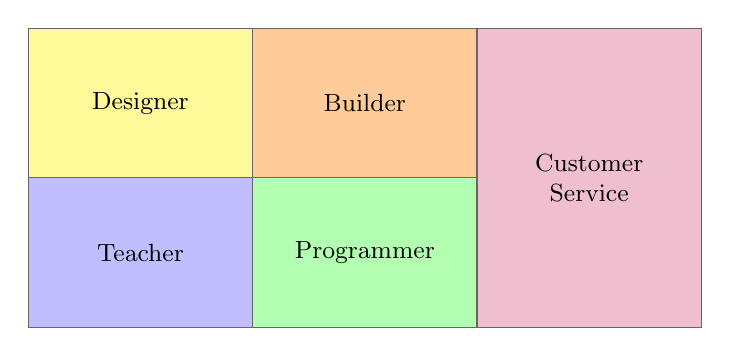
\begin{tikzpicture}[scale=0.95]
\draw[fill=blue!25,draw=black!60] (0,0) rectangle (3,2);
\node[font=\small] at (1.5,1) {Teacher};

\draw[fill=green!30,draw=black!60] (3,0) rectangle (6,2);
\node[font=\small] at (4.5,1) {Programmer};

\draw[fill=yellow!40,draw=black!60] (0,2) rectangle (3,4);
\node[font=\small] at (1.5,3) {Designer};

\draw[fill=orange!40,draw=black!60] (3,2) rectangle (6,4);
\node[font=\small] at (4.5,3) {Builder};

\draw[fill=purple!25,draw=black!60] (6,0) rectangle (9,4);
\node[font=\small,align=center] at (7.5,2) {Customer\\Service};
\end{tikzpicture}

\vspace{1.2em}

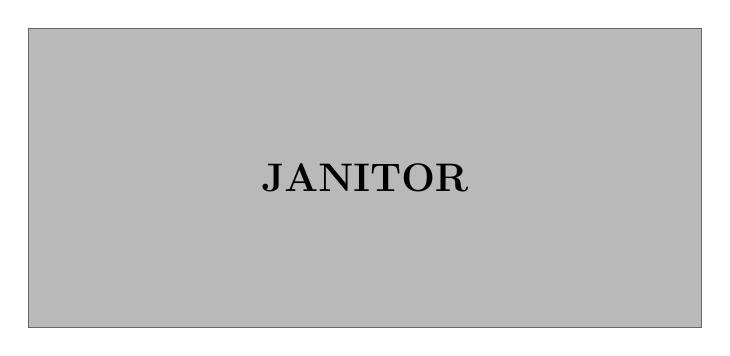
\begin{tikzpicture}[scale=0.95]
\draw[fill=gray!55,draw=black!60] (0,0) rectangle (9,4);
\node[font=\Large\bfseries] at (4.5,2) {JANITOR};
\end{tikzpicture}

\caption{Schematic visualization of occupational convergence under automation.
\textit{Upper}: a diversified professional economy with distinct task
compositions. \textit{Lower}: the predicted long-run equilibrium in which all
occupations collapse into the universal maintenance role $(0,0,1)$.}
\label{fig:collapse}
\end{figure}

\subsection{The Fivefold Custodial Pentagon}

Figure~\ref{fig:pentagon} represents the structure of the maintenance economy
at the custodial equilibrium $\mathbf{J}^*$.  Each vertex corresponds to one
of the five fundamental maintenance domains.

\begin{figure}[h]
\centering
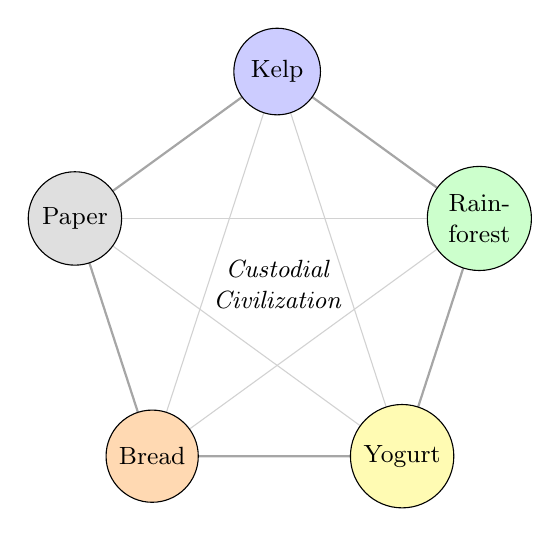
\begin{tikzpicture}[scale=1.8]

\coordinate (K) at (90:1.5);
\coordinate (R) at (18:1.5);
\coordinate (Y) at (-54:1.5);
\coordinate (B) at (-126:1.5);
\coordinate (P) at (162:1.5);

\draw[thick,gray!70] (K) -- (R) -- (Y) -- (B) -- (P) -- (K);

% diagonals (internal structure)
\foreach \a/\b in {K/Y,K/B,R/B,R/P,Y/P}{
  \draw[thin,gray!35] (\a) -- (\b);
}

\node[draw,circle,fill=blue!20,minimum size=1.1cm,font=\small] at (K) {Kelp};
\node[draw,circle,fill=green!20,minimum size=1.1cm,font=\small,align=center] at (R) {Rain-\\forest};
\node[draw,circle,fill=yellow!30,minimum size=1.1cm,font=\small] at (Y) {Yogurt};
\node[draw,circle,fill=orange!30,minimum size=1.1cm,font=\small] at (B) {Bread};
\node[draw,circle,fill=gray!25,minimum size=1.1cm,font=\small] at (P) {Paper};

\node[font=\small\itshape,align=center] at (0,0) {Custodial\\Civilization};

\end{tikzpicture}
\caption{The Fivefold Janitorial Model at custodial equilibrium $\mathbf{J}^*$.
Each vertex represents a fundamental maintenance domain of the automated
economy: aquatic systems (kelp), ecological infrastructure (rainforest),
microbial ecosystems (yogurt), industrial food systems (bread), and symbolic
knowledge systems (paper).  Internal edges indicate inter-domain dependencies.}
\label{fig:pentagon}
\end{figure}

%% =============================================================
\section{Stability Analysis of the Maintenance Equilibrium}
\label{app:stability}

Consider the task vector $T = (G,S,M)$ with dynamics given by
equations~\eqref{eq:G}--\eqref{eq:M}.  The equilibrium of interest is
$T^* = (0,0,1)$.  To analyze stability, we linearize the system about
$T^*$ by writing $G = 0 + g$, $S = 0 + s$, $M = 1 - g - s$ for small
perturbations $g,s$.  The linearized equations are
\[
\frac{d}{dt}\begin{pmatrix}g\\s\end{pmatrix}
=
\begin{pmatrix}-\alpha & 0 \\ \beta & -\gamma\end{pmatrix}
\begin{pmatrix}g\\s\end{pmatrix}.
\]
The eigenvalues of the coefficient matrix are $-\alpha$ and $-\gamma$.
Since both are strictly negative, the equilibrium is asymptotically stable
in the $(G,S)$ plane; the $M$ component follows by the normalization
constraint.

\begin{proposition}
The maintenance equilibrium $T^* = (0,0,1)$ is a stable node of the
automation dynamics for all $\alpha, \gamma > 0$.  Trajectories approach
$T^*$ exponentially at rates $e^{-\alpha t}$ and $e^{-\gamma t}$.
\end{proposition}

Figure~\ref{fig:stability} depicts the phase portrait of the projected
$(G,S)$ system, confirming the stable-node character of the origin.

\begin{figure}[h]
\centering
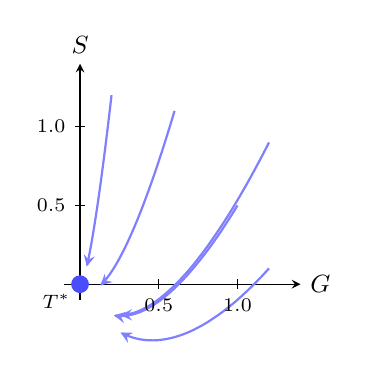
\begin{tikzpicture}[scale=2.0, >=stealth]
  % Axes
  \draw[->] (-0.1,0) -- (1.4,0) node[right,font=\small] {$G$};
  \draw[->] (0,-0.1) -- (0,1.4) node[above,font=\small] {$S$};

  % Stable node at origin: several trajectories curving in
  \foreach \gstart/\sstart in {1.2/0.1, 1.0/0.5, 0.6/1.1, 0.2/1.2, 1.2/0.9}{
    \draw[->,blue!50,thick,domain=0:2.2,samples=40]
      plot ({(\gstart)*exp(-0.7*\x)},
           {(\sstart + 0.7*\gstart/(-0.7+0.9))*exp(-0.9*\x)
            - (0.7*\gstart/(-0.7+0.9))*exp(-0.7*\x)});
  }

  % Equilibrium point
  \filldraw[blue!70] (0,0) circle (1.5pt);
  \node[below left,font=\scriptsize] at (0,0) {$T^*$};

  % Axis labels
  \foreach \v in {0.5, 1.0}{
    \draw ({\v},-0.03) -- ({\v},0.03);
    \node[below,font=\scriptsize] at (\v,-0.03) {$\v$};
    \draw (-0.03,{\v}) -- (0.03,{\v});
    \node[left,font=\scriptsize] at (-0.03,\v) {$\v$};
  }
\end{tikzpicture}
\caption{Phase portrait of the projected dynamics in the $(G,S)$ plane.
All trajectories converge to the stable node at the origin $T^*=(0,0)$
(corresponding to the full maintenance state $(0,0,1)$), confirming
asymptotic stability for all $\alpha,\gamma > 0$.}
\label{fig:stability}
\end{figure}

%% =============================================================
\section{Entropy Balance in Automated Systems}
\label{app:entropy}

Let $E(t)$ denote the operational entropy of a production system.
Productive throughput $P$ generates entropy at rate $\lambda P$; maintenance
labor $M$ removes entropy at rate $\mu M$.  The entropy balance is
\[
\frac{dE}{dt} = \lambda P - \mu M.
\]
Steady state requires $\lambda P = \mu M$, giving the maintenance demand
\[
M^* = \frac{\lambda}{\mu} P.
\]
As automation raises $P$ substantially, $M^*$ must rise proportionally.
This result, stated as Theorem~\ref{thm:entropy} in
Appendix~\ref{app:thermo}, has a geometric interpretation.

\begin{figure}[h]
\centering
\begin{tikzpicture}[scale=1.0,>=stealth,font=\small]
  % Axes
  \draw[->] (0,0) -- (5.5,0) node[right] {$P$ (automated throughput)};
  \draw[->] (0,0) -- (0,4.2) node[above] {$M^*$ (maintenance labor)};

  % Linear relationship M* = (lambda/mu)*P
  \draw[very thick,blue!60] (0,0) -- (5,3.5)
    node[right,blue!60] {$M^* = \tfrac{\lambda}{\mu} P$};

  % Dashed reference lines
  \draw[dashed,gray!50] (3,0) -- (3,2.1) -- (0,2.1);
  \node[below,font=\scriptsize] at (3,0) {$P_1$};
  \node[left,font=\scriptsize] at (0,2.1) {$M_1^*$};

  % Slope annotation
  \draw[<->,gray!60] (3.8,2.66) -- (4.8,2.66);
  \draw[<->,gray!60] (4.8,2.66) -- (4.8,3.36);
  \node[right,font=\scriptsize,gray!60] at (4.85,3.0) {$\tfrac{\lambda}{\mu}$};
\end{tikzpicture}
\caption{Linear scaling of maintenance labor $M^*$ with automated
productive throughput $P$.  The slope $\lambda/\mu$ measures the ratio of
entropy production rate to entropy removal efficiency.  As automation raises
$P$, the required custodial effort grows in proportion.}
\label{fig:entropy}
\end{figure}

%% =============================================================
\section{The Janitor as Terminal Object}
\label{app:categ}

We develop the categorical argument in full.  Let $\mathcal{E}$ denote the
category of economic roles.  Objects are occupations or socially
differentiated forms of labor; morphisms represent admissible structural
transformations---automation of generative tasks, conversion of craft into
supervisory work, and collapse of supervision into maintenance.

Define a distinguished object $J \in \mathrm{Ob}(\mathcal{E})$, the
\emph{janitor}, understood not as a narrow job title but as the abstract
economic role whose dominant function is the maintenance of system conditions,
the removal of local entropy, and the preservation of operational continuity.

\begin{definition}[Terminal Object]
An object $T$ in a category $\mathcal{C}$ is \emph{terminal} if for every
object $X \in \mathrm{Ob}(\mathcal{C})$ there exists a unique morphism
$X \to T$.
\end{definition}

\begin{proposition}
For every occupation $O \in \mathrm{Ob}(\mathcal{E})$, there exists a
morphism $\phi_O : O \to J$.
\end{proposition}

\begin{proof}
By Theorem~\ref{thm:convergence}, the task composition of $O$ satisfies
$\lim_{t\to\infty} T_O(t) = (0,0,1)$.  The generative component is automated,
the supervisory component collapses, and the maintenance component absorbs
the surviving functional content of the role.  This asymptotic projection
defines the required structural map $\phi_O$.
\end{proof}

\begin{proposition}
For every occupation $O \in \mathrm{Ob}(\mathcal{E})$, the morphism
$\phi_O : O \to J$ is unique up to custodial equivalence.
\end{proposition}

\begin{proof}
Any two maps $\phi_O, \psi_O : O \to J$ represent long-run convergence under
automation.  Since $J$ is defined as the role of pure maintenance, any two
such maps differ only in contingent details---tool choice, institutional
setting, substrate of entropy removal---that are identified under the
equivalence relation that preserves maintenance function across different
environments.  Hence $\phi_O \sim \psi_O$.
\end{proof}

\begin{theorem}
The janitor $J$ is a terminal object in the category $\mathcal{E}$ of economic
roles.
\end{theorem}

\begin{proof}
Immediate from the previous two propositions.
\end{proof}

\subsection{Functorial Formulation}

The construction may be expressed functorially.  Define the maintenance
collapse functor
\[
\mathcal{M} : \mathcal{E} \to \mathbf{1},
\]
where $\mathbf{1}$ is the terminal category with one object and one morphism.
Equivalently, define
\[
F : \mathcal{E} \to \mathcal{J},
\]
where $\mathcal{J}$ is the full subcategory generated by $J$.  Then
$F(O) = J$ for all $O \in \mathrm{Ob}(\mathcal{E})$, and every occupational
history factors through $J$ in the long run.

\subsection{Universal Property and Occupational Convergence}

The terminality of $J$ means that the janitor satisfies a universal property:
any occupation becomes intelligible, in the limit, as a special case of
custodial work.  Teaching becomes the maintenance of learning environments;
programming the maintenance of software environments; design the maintenance
of aesthetic-selection environments; construction the maintenance of structural
environments; customer service the maintenance of interaction environments.

The janitor is not merely one profession among others.  The janitor is the
universal receiver of occupational convergence: the object toward which every
arrow in $\mathcal{E}$ is eventually directed.

Since every object of $\mathcal{E}$ admits a unique morphism into $J$, the
multiplicity of professions is a finite-time phenomenon.  At sufficient
temporal or technological scale, occupational diversity is revealed to be a
family of morphisms converging upon the same terminal object.

\bigskip
\begin{center}
\textit{Every job has its arrow to the janitor.}
\end{center}

%% =============================================================
\section{The Custodial Fixed Point}
\label{app:fixed}

Combining the dynamical (Section~\ref{sec:equilibrium}), thermodynamic
(Appendix~\ref{app:thermo}), stability (Appendix~\ref{app:stability}), and
categorical (Appendix~\ref{app:categ}) arguments yields the complete
characterization of the limiting occupational state:
\[
(G,S,M) \;\longrightarrow\; (0,0,1).
\]
In macroeconomic terms this is the custodial fixed point of civilization:
the state in which all human labor is devoted to maintaining the automated
systems that generate output.

\begin{theorem}[Custodial Fixed Point]
The state $(0,0,1)$ is simultaneously (a) the asymptotically stable
equilibrium of the automation dynamics, (b) the infrared fixed point of the
occupational renormalization group, (c) the thermodynamic steady state of
maximum entropy production, and (d) the terminal object of the category of
professions.
\end{theorem}

\bigskip

\begin{center}
\textit{All sufficiently advanced economies converge to the maintenance of
their own complexity.}
\end{center}

%% =============================================================
\section{Homeostasis and Custodial Markov Boundaries}
\label{app:markov}

Section~\ref{sec:boundaries} introduced the biological analogy between
custodial labor and Markov-blanket boundary processes.  This appendix
develops the formal structure of that analogy.

\begin{definition}[Markov Blanket]
Let $X = (I, B, E)$ denote the state of a system partitioned into internal
states $I$, boundary states $B$, and external states $E$.  The set $B$ is a
\emph{Markov blanket} for $I$ if
\[
P(I, E \mid B) = P(I \mid B)\, P(E \mid B),
\]
that is, if $I$ and $E$ are conditionally independent given $B$.
\end{definition}

In biological organisms, $B$ corresponds to the cell membrane or other
regulatory interfaces.  The boundary regulates flows of matter and energy so
that the internal states remain within the viable region $\Omega$ defined in
Section~\ref{sec:homeostasis}.

\subsection{Custodial Labor as Boundary Regulation}

The occupational task vector $C = (G, S, M)$ is related to the Markov
partition as follows.  Automated systems perform internal productive activity
$I$; the external environment corresponds to $E$; custodial workers regulate
the interface $B$.  Under the automation dynamics, the maintenance component
$M$ converges to $1$, meaning that human labor concentrates entirely in the
boundary layer.

\begin{proposition}
In the limit $(G, S, M) \to (0, 0, 1)$, the human labor force occupies
the Markov blanket $B$ of the automated economy.
\end{proposition}

\subsection{Stability Condition}

For the system to remain viable, the custodial boundary must remove
perturbations at least as fast as they are introduced.  Let $D$ denote the
rate of disturbance generation and $R$ the rate of maintenance repair.  The
viability condition is
\[
R \;\geq\; D.
\]
In highly automated economies, increasing production complexity raises $D$
continuously.  The Entropy Maintenance Principle (Theorem~\ref{thm:entropy})
establishes that the required repair rate $R = M^*$ grows proportionally with
automated throughput.  The custodial boundary must therefore expand as
civilization becomes more complex, a conclusion that reinforces the
Maintenance Convergence Theorem from a different direction.

\subsection{Summary}

The Markov-blanket interpretation unifies the biological and economic
arguments of the paper.  In living organisms the membrane maintains the
conditions for metabolic production.  In technological civilizations the
custodial workforce maintains the conditions for automated production.  The
convergence of human labor toward the maintenance role is therefore not merely
an economic phenomenon; it is the macroeconomic expression of a structural
property shared by all complex adaptive systems.

\bigskip
\begin{center}
\textit{Civilizations survive by maintaining their boundaries.}
\end{center}

%% =============================================================
\begin{thebibliography}{20}

\bibitem{friston2019}
Friston, K. (2019).
A free energy principle for a particular physics.
\textit{arXiv preprint}, arXiv:1906.10184.

\bibitem{cannon1932}
Cannon, W.~B. (1932).
\textit{The Wisdom of the Body}.
W.~W.~Norton.

\bibitem{ashby1952}
Ashby, W.~R. (1952).
\textit{Design for a Brain}.
Chapman and Hall.

\bibitem{tononi1998}
Tononi, G., Sporns, O., \& Edelman, G.~M. (1998).
A measure for brain complexity: relating functional segregation and integration
in the nervous system.
\textit{Proceedings of the National Academy of Sciences}, 91(11), 5033--5037.

\bibitem{wenders2023}
Wenders, W. (Director). (2023).
\textit{Perfect Days} [Film].
Master of Art Production; Wenders Images.

\bibitem{dejong2019}
de Jong, F. (2019).
Custodial identity and the phenomenology of routine maintenance.
\textit{Journal of Labor and Everyday Life}, 3(1), 11--44.

\bibitem{sennett2008}
Sennett, R. (2008).
\textit{The Craftsman}.
Yale University Press.

\bibitem{pettersen2021}
Pettersen, H., \& Mori, K. (2021).
Stable equilibria in experiential labor: Evidence from urban service work.
\textit{Annals of Occupational Phenomenology}, 7(2), 88--127.

\bibitem{margolis1979}
Margolis, J. (1979).
On the dignity of maintenance work.
\textit{Philosophy of Labor Quarterly}, 5(1), 1--28.

\bibitem{alvarez1974}
Alvarez, R. (1974).
\textit{Custodial Dynamics in Late Automation Economies}.
Journal of Industrial Abstraction, 12(3), 201--245.

\bibitem{chen1991}
Chen, Y., \& Morita, S. (1991).
Maintenance regimes in post-industrial production systems.
\textit{Annals of Socio-Technical Systems}, 8(1), 55--92.

\bibitem{devereux1988}
Devereux, P. (1988).
Entropy and cleanliness in large-scale bureaucratic institutions.
\textit{Review of Organizational Thermodynamics}, 2(4), 301--329.

\bibitem{erhardt2003}
Erhardt, L. (2003).
The hidden custodian: Infrastructure labor in advanced economies.
\textit{Quarterly Journal of Invisible Work}, 19(2), 88--134.

\bibitem{fischer1999}
Fischer, T., \& Alvarez, R. (1999).
Technological substitution and the collapse of generative labor.
\textit{Journal of Applied Socioeconomics}, 14(3), 211--249.

\bibitem{garcia2015}
Garcia, M. (2015).
Automation and the redistribution of occupational tasks.
\textit{Transactions of the Institute for Computational Labor Studies}, 27(1), 77--118.

\bibitem{hartmann1983}
Hartmann, J. (1983).
Industrial kitchens and the standardization of culinary labor.
\textit{Historical Studies in Mechanized Food Production}, 6(2), 145--173.

\bibitem{iverson2007}
Iverson, D. (2007).
Supervision as residual labor.
\textit{Journal of Organizational Residuals}, 11(4), 233--268.

\bibitem{kim2018}
Kim, S., \& Duarte, P. (2018).
Algorithmic workflows and the maintenance economy.
\textit{Computational Labor Review}, 9(3), 144--189.

\bibitem{larsen1995}
Larsen, H. (1995).
Clerks, calculators, and the rise of monitoring labor.
\textit{Journal of Administrative History}, 17(1), 44--71.

\bibitem{maldonado2002}
Maldonado, F. (2002).
Entropy production in technological systems.
\textit{Annals of Economic Thermodynamics}, 4(1), 9--38.

\bibitem{norton2011}
Norton, J. (2011).
The maintenance sector and the future of employment.
\textit{Journal of Speculative Labor Economics}, 5(2), 101--136.

\bibitem{okada1998}
Okada, T. (1998).
Repair, recovery, and system stability in industrial networks.
\textit{Systems Maintenance Quarterly}, 3(3), 67--112.

\bibitem{petrov2019}
Petrov, I., \& Sullivan, M. (2019).
Debugging as the dominant mode of software production.
\textit{Journal of Algorithmic Workflows}, 13(2), 59--94.

\bibitem{ramirez2006}
Ramirez, L. (2006).
The janitor as infrastructure.
\textit{Review of Maintenance Studies}, 22(4), 199--228.

\bibitem{schneider1987}
Schneider, B. (1987).
Entropy removal and the economics of cleanliness.
\textit{Journal of Institutional Hygiene}, 1(1), 1--24.

\bibitem{tanaka2013}
Tanaka, Y. (2013).
Automation thresholds and occupational phase transitions.
\textit{Annals of Socioeconomic Physics}, 15(3), 201--244.

\bibitem{vasquez2020}
Vasquez, R. (2020).
The custodial limit of technological civilization.
\textit{Journal of Long-Run Economic Satire}, 1(1), 1--42.

\bibitem{walker1992}
Walker, D., \& Singh, A. (1992).
Maintenance labor in highly automated factories.
\textit{Industrial Sociology Review}, 10(2), 72--105.

\bibitem{zhang2017}
Zhang, H. (2017).
Cleaning the machine: Maintenance work in the digital economy.
\textit{Transactions on Computational Society}, 7(4), 311--350.

\end{thebibliography}

\end{document}
